% Created 2020-08-26 Wed 20:47
% Intended LaTeX compiler: pdflatex
\documentclass[11pt]{article}
\usepackage[utf8]{inputenc}
\usepackage[T1]{fontenc}
\usepackage{graphicx}
\usepackage{grffile}
\usepackage{longtable}
\usepackage{wrapfig}
\usepackage{rotating}
\usepackage[normalem]{ulem}
\usepackage{amsmath}
\usepackage{textcomp}
\usepackage{amssymb}
\usepackage{capt-of}
\usepackage{hyperref}
\usepackage{graphicx}
\usepackage{longtable}
\usepackage{float}
\setlength{\parindent}{1em}
\setlength{\parskip}{0.5em}
\usepackage[citestyle=alphabetic,bibstyle=alphabetic, hyperref=true, backref=true,maxcitenames=3,url=true,backend=biber,natbib=true, maxbibnames=9] {biblatex}
\addbibresource{bibliography.bib}
\usepackage[a4paper, total={7in, 9in}]{geometry}
\usepackage[font={small, it},labelfont=bf]{caption}
\usepackage[ruled, procnumbered]{algorithm2e}
\usepackage{listings}
\SetArgSty{}
\usepackage[dvipsnames]{xcolor}
\usepackage{amssymb}
\usepackage{pifont}
\newcommand{\cmark}{\color{ForestGreen}\ding{52}}%
\newcommand{\xmark}{\color{Maroon}\ding{55}}%
\hypersetup{colorlinks=true}
\renewcommand{\sectionautorefname}{{\color{Black}\S}}
\renewcommand{\subsectionautorefname}{{\color{Black}\S\S}}
\renewcommand{\subsubsectionautorefname}{{\color{Black}\S\S\S}}
\renewcommand{\functionautorefname}{{\color{Black}\textbf{Function}}\color{Magenta}}
\renewcommand{\algorithmautorefname}{{\color{Black}\textbf{Algorithm}}\color{Magenta}}
\usepackage{subcaption}
\usepackage[shortlabels]{enumitem}
\usepackage{newfloat}
\DeclareFloatingEnvironment[fileext=lol, listname={List of Iterated Function System definitions}, name=IFS, placement=tbhp, within=section]{ifs}
\usepackage{wrapfig}
\usepackage{todonotes}
\usepackage{pifont,kantlipsum}
\newcommand*{\altasterism}{\vspace*{1em plus .5em minus .5em}\noindent\hspace*{\fill}\ding{104}\hspace*{\fill}}
\usepackage{rugscriptie}
\supervisor{dr. J. Kosinka}
\supervisor{G. J. Hettinga}
\date{August 2020}
\faculty{fse} % Or feb, fgg, fgmw, fl, frg, frw, fw, umcg
\thesistype{Bachelor's thesis} % Will be printed unmodified
\author{Wiebe-Marten Wijnja}
\date{\today}
\title{\Huge In by Out Again\\\medskip
\large Arbitrarily-Deep Zooming on Iterated Function Systems by `Self-Similarity Jumping'}
\hypersetup{
 pdfauthor={Wiebe-Marten Wijnja},
 pdftitle={\Huge In by Out Again},
 pdfkeywords={},
 pdfsubject={},
 pdfcreator={Emacs 26.3 (Org mode 9.3.6)}, 
 pdflang={English}}
\begin{document}

\maketitle
\setcounter{tocdepth}{4}
\tableofcontents

\listoftodos

\todo[inline]{Turn off todo list}

\pagebreak

\section*{Abstract}
\label{sec:orgd88de45}
Iterated Function Systems (IFSs) are a mathematical concept which, amongst other uses, 
is used for rendering fractals that sees wide usage in the modeling of physical phenomena, 
image compression, and the creation of abstract art.
When exploring an IFS interactively, current IFS rendering techniques require a full re-approximation of the IFS's attractor at every frame.

This thesis proposes a combination of two techniques to enable faster exploring of IFSs.
First, a point cloud is used as an intermediate attractor approximation, that can be re-used between animation frames.
Secondly, a technique coined 'self-similarity jumping' is proposed to keep the attractor representation detailed, even when zooming in very far.

A proof-of-concept computer program has been implemented
which shows that the employed techniques, while promising, 
are somewhat restricted in their usefullness because self-similarity jumping cannot be used in all situations.

\pagebreak

\section{Introduction}
\label{sec:orgeaf20a7}

Iterated Function Systems (IFSs) are a mathematical concept which, amongst other uses, is used to generate infinitely detailed fractal images 
by repeatedly applying simple mathematical functions until a fixed point is reached \cite{barnsley1988fractals}. 
IFSs see use in the modeling and rendering of physical phenomena, image compression \cite{hart1996fractal} and representing gene structures \cite{jeffrey1990chaos}.
Sometimes they also are used plainly for the aesthetic beauty of their graphical representations \cite{draves2003fractal}.

Various computer algorithms to visualize IFSs exist \cite{hepting1991rendering}.
However, these all take a single still image as final result. If these algorithms are employed to render an animation,
this animation is treated as a sequence of completely separate still images.

This leaves a venue for potential optimization: if there is information that remains the same between animation frames, 
then we could compute this information only once and re-use it for all frames.

For instance, many kinds of animations consist of transformations of the camera viewport w.r.t the viewed fractal over time like translation, rotation and scaling. 
These transformations do not require alterations to the fractal itself.
This means that (an approximation of) the fractal might be computed once and then be used for all frames.

Furthermore, because of the self-similar nature of the rendered fractals,
it might be possible to simulate zooming in to an arbitrary depth by `jumping up' to a more shallow camera viewport
that shares the same self-similarity as the original camera viewport.

This thesis is an in-depth investigation of these two ideas.

\subsection{Overview}
\label{sec:orga5b2460}

In the next section, \autoref{section:background}, Iterated Function Systems are introduced and pre-existing methods to render their attractors in single-threaded and heavily parallel environments described.
This then leads to a clear definition of the research question in \autoref{section:research_question}.
The approach taken to test this question is described in \autoref{section:approach}, followed by a qualitative discussion of the results in \autoref{section:findings}.
We conclude in \autoref{section:conclusion} and finally hint at some approaches for further work in \autoref{section:further_work}.

\section{Background}
\label{sec:orgd84a6d8}
\label{section:background}

This section describes the different building blocks necessary to formulate the research question.
First, IFSs are formalized, followed by a description of the different ways in which an IFS's attractor can be rendered, 
and how these techniques might be parallellized.

\subsection{Informal description of an Iterated Function System}
\label{sec:org4f51759}
\label{subsection:informal_description}

\begin{figure}
\centering
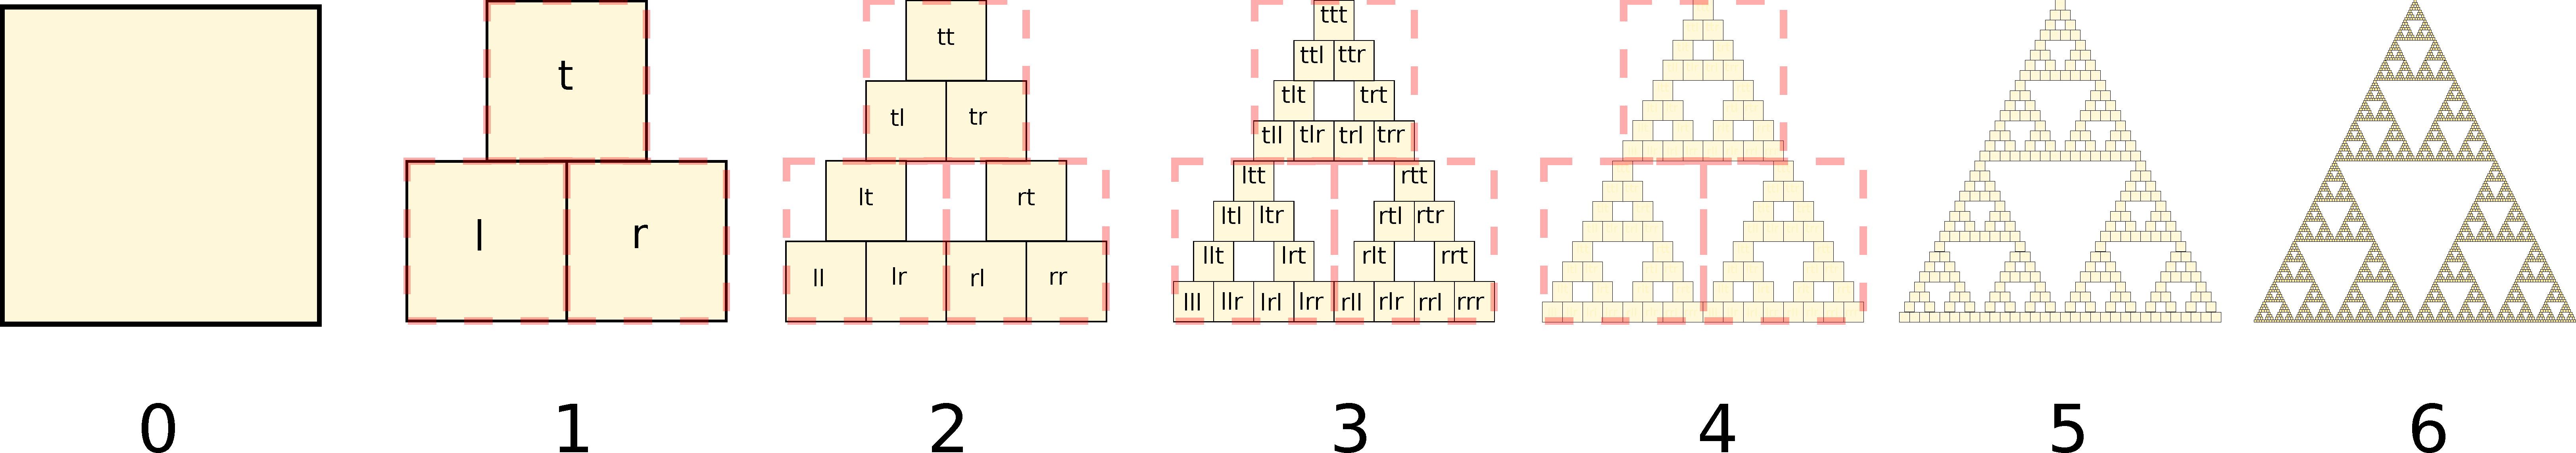
\includegraphics[width=\textwidth]{figures/sierpinsky_iterations}
\caption{The first six iterations of the Sierpi\'nsky triangle IFS (\autoref{ifs:sierpinsky}). 
The initial image is just the unit square. We then iteratively combine the results of transforming the current image using one of the three mappings. 
The letters indicate which (sequence of) transformation(s) resulted in this part of the image.
Dashed red lines are used for the first four iterations to indicate the self-similarity between the previous iteration and the current one extra clearly.
Already after a couple of iterations it can be seen that the shape of the original image has no influence on the shape of the attractor.}
\label{figure:sierpinsky_iterations}
\end{figure}


Informally, an Iterated Function System is a set of mappings (transformation functions) that, given any input image, create a new image by

\begin{enumerate}
\item transforming the input image with each of the transformations;
\item overlaying all transformed images, forming one new image that is the combination (union) of the transformed images. This is the new image.
\end{enumerate}

This process is then repeated an arbitrary number of times, until changes between the input image and new image are no longer visible to the human eye.

The image you end up with is a visual representation of the IFS's attractor.
A simple example of this process can be seen in \autoref{figure:sierpinsky_iterations}.



\subsection{Formal definition of an Iterated Function System}
\label{sec:orgc0cbde3}
\label{subsection:formal_ifs_definition}

Formally, an Iterated Function System \(F\) consists of a finite set of contraction mappings that map a complete metric space\footnote{A metric space is a set \(\mathcal{M}\) together with a \emph{metric} \(d(x, y)\) on that set . The metric is a function that for any two elements (or `points') in \(\mathcal{M}\) returns the `distance' between them, for any notion of distance adhering to the `identity of indiscernibles' (\(d(x, y)  = 0 \Leftrightarrow x = y\)), `symmetry' (\(d(x, y) = d(y, x)\)) and `triangle inequality' (\(d(x, z) \leq d(x, y) + d(y, z)\)) properties. Often, \(d\) is elided and just \(\mathcal{M}\) is used to refer to the metric space when it is clear from context which metric is used.} \((\mathcal{M}, d)\) to itself \cite{barnsley1988fractals}:

$$ \mathcal{F} = \{ f_i : \mathcal{M} \rightarrow \mathcal{M}\}_{i=1}^N, N \in \mathbb{N}.$$

All mappings are required to be contractive. This means that for each mapping \(f_i\), the distance between every two arbitrary points \(a\) and \(b\) in \((\mathcal{M}, d)\) 
needs to be larger than the distance of these points after transforming them:

$$\forall i \bigl( d(f_i(a), f_i(b)) < d(a, b) \bigr).$$

We can then take the union of performing all of these mappings on any compact set of points \(\mathcal{S}_0 \subset \mathcal{M}\). This procedure is called the \emph{Hutchkinson Operator} and denoted \(H\).
It can be iterated as many times as desired:

$$ \mathcal{S}_{n + 1} = H(\mathcal{S}_n) = \bigcup_{i=1}^{N} f_i(\mathcal{S}_n), n \in \mathbb{N}.$$

When performed an arbitrary number of times, the fixed-point or attractor, \(\mathcal{A}\), of \(\mathcal{F}\) is approached:

$$\mathcal{A} = \lim_{n \rightarrow \infty} \mathcal{S}_n.$$

Curiously, which set of points \(\mathcal{S}_0\) we picked does not influence the shape of \(\mathcal{A}\) \cite{mendivil2003fractals}. We might even start with a single point (denoted \(z_0\)).

\subsubsection{Restriction to affine transformations on the two-dimensional Euclidean plane}
\label{sec:orgf7f5f53}

IFSs are traditionally using \(\mathbb{R}^2\) as metric space\footnote{More formally, the two-dimensional Euclidean space: \(\left(\mathbb{R}^2, d(p, q) = \sqrt{(p - q)^2}\right)\).} (which can easily be rendered to screen or paper),
and only use \emph{affine transformations} as mappings.

It is very practical to work in this restricted scenario 
and potentially generalize obtained results to a wider number of scenarios later.
Therefore, these are also the restrictions that will be used in this thesis.

\subsubsection{The viewport transformation}
\label{sec:orgc228070}
\label{subsection:viewport_transformation}

When rendering graphics, we view the world through a (virtual) \emph{camera} which has a particular frustum 
that limits what parts of the world (in this case the IFS's attractor) end up on the \emph{viewport}.

\begin{enumerate}
\item Scaling vs zooming
\label{sec:org89ea1ba}

Because of the presence of a camera, the part of an object that will be visible in the camera viewport may change when scaling said object.
We use the term `zooming' to disambugate this type of scaling where a camera is present.

\item Freedom of choosing an initial camera position and frustum
\label{sec:org24aebeb}

For any IFS we can transform its attractor by any invertible map \(t\) by adjusting each of the IFS's mappings according to the
transform theorem, defined as \(f_i' = t \circ f_i \circ t^{-1}\) \cite{barnsley1988fractals}. 
Essentially points are transformed from the new (program-desired) space to the old (user-supplied) space, then the mapping is applied, and finally the points are transformed back to the new space.
This allows users the freedom to choose any desired mappings together with an `initial camera transformation' (i.e. the camera's initial position + frustum),
while still allowing all calculations to happen with regard to the unit square (`unit space'), keeping them simple.
\end{enumerate}

\subsection{Rendering an Iterated Function System}
\label{sec:orgf5cc6a6}

A couple of algoritms (\cite{barnsley1988fractals}, \cite{hepting1991rendering}, \cite{lawlor2012gpu}) exist to render the attractor of an Iterated Function System. 
It is impossible to render the attractor exactly, as this would require an infinite number of transformation steps.
However, in practice we can stop applying transformation steps when the difference between our approximation and the attractor is smaller than
the smallest detail we can visually distinguish (e.g. when rendering to a screen, smaller than the size of a pixel).
The number of iterations (i.e. transformations) to reach this point we call \(k\)\footnote{It is possible to calculate \(k\) precisely if you know the precision of your canvas and the `contraction factor' of the IFS. C.f. \cite{barnsley1988fractals}.}.

Therefore, to render the attractor approximation on a computer, 
we have to look up all possible sequences of transformations of length \(k\),
and then take the union of applying all of these sequences to our initial image\footnote{As already mentioned in \autoref{subsection:formal_ifs_definition}, we usually take a single point \(z_0\) as input image for simplicity. In other words, \(S_0 = \{z_0\}\).}.

The difficult part here is to gather all possible \(k\)-length transformation-sequences.

More in-depth information about the rendering of Iterated Function Systems can be found in \cite{hepting1991rendering}. 
Short summaries of the two most common techniques now follow.

\subsubsection{The deterministic method}
\label{sec:orga8bb6ed}

One way of looking at this problem, is to consider all possible transformation-combinations together as an (infinite) tree\footnote{An in-depth description of what trees are and how the various tree-traversals that are briefly mentioned work is outside of the scope of this thesis as the deterministic method that uses trees is itself only mentioned for the sake of comparison with the new approach that is based on the chaos game.
We refer to \cite{hepting1991rendering} for a deeper understanding of trees, tree traversals and the deterministic method of rendering IFS attractors.}.
We now only have to traverse this tree up to the depth \(k\).

The algorithm works as follows:

\begin{enumerate}
\item Pick a starting point \(z_0\);
\item traverse the tree down to the chosen depth \(k\), keeping track of the traversed sequence of transformations \footnote{\(\circ\) stands for function composition: \((f \circ g)(x) = f(g(x))\). 
Be aware that when affine transformation functions are represented as matrices (e.g. \(F\) and \(G\)), 
the matrix premultiplication resulting in the same transformation is in the opposite order (\(f \circ g \Leftrightarrow G \cdot F\)).} \(f_{i_k} \circ \ldots \circ f_{i_1}\);
\item for each node at this depth, evaluate and render \(z_k = (f_{i_k} \circ \ldots \circ f_{i_1})(z_0) = f_{i_k-1}(z_{k-1})\).
\end{enumerate}

Since \(z_{k} = f_{i_k-1}(z_{k-1})\) this procedure takes, for an approximation that consists of \(P\) points, depending on the tree traversal chosen:

\begin{itemize}
\item a linear amount of memory ( \(\mathcal{O}(P)\) ) for a breadth-first tree-traversal\footnote{For any breadth-first traversal, we need to keep track of all nodes that have not been expanded deep enough, therefore the linear amount of memory required.};
\item a logarithmic amount of memory ( \(\mathcal{O}(\log{P})\) ) for a depth-first tree-traversal\footnote{For any depth-first traversal, we (only) need to keep track of all parents of the current node, to go back up to the current node's parent once this node's subtree was fully traversed. Therefore, only a logarithmic amount of memory is required.}.
\end{itemize}

One advantage of the breadth-first traversal is that the rendering process can be stopped interactively,
while the depth-first traversal requires the stopping criterion to be known beforehand \cite{hepting1991rendering}.

Both kinds of traversals take a linear amount of time ( \(\mathcal{O}(N \cdot P) \approx \mathcal{O}(P)\), where \(N\) is the number of mappings the IFS consists of).

While the deterministic method is easy to understand (and indeed is a direct implementation of the informal process described in \autoref{subsection:informal_description}),
it is usually less efficient and more complex to implement on a computer than the algorithm that is described next.

\subsubsection{The chaos game}
\label{sec:org3d53d73}
\label{subsection:chaos_game}

\begin{figure}
     \centering
     \begin{subfigure}[b]{0.4\textwidth}
         \centering
         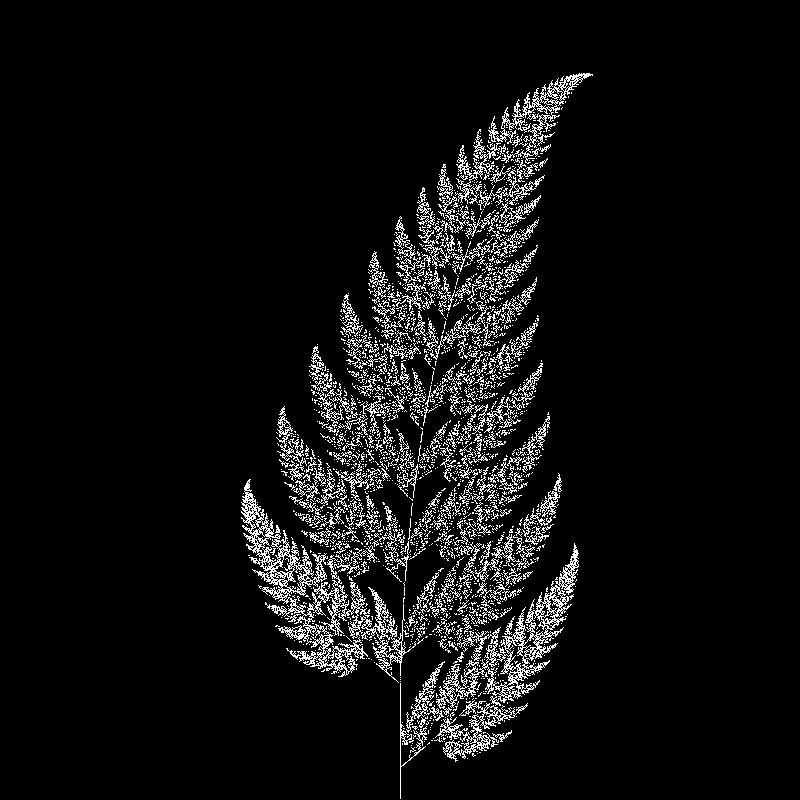
\includegraphics[width=\textwidth]{figures/barnsley_1000000}
         \caption{1,000,000}
         \label{figure:barnsley_mil}
     \end{subfigure}
     \hfill
     \begin{subfigure}[b]{0.4\textwidth}
         \centering
         
\includegraphics[width=\textwidth]{figures/barnsley_100000000}
         \caption{10,000,000}
         \label{figure:barnsley_ten_mil}
     \end{subfigure}
        \caption{The Barnsley Fern (\autoref{ifs:barnsley_fern}), rendered using the chaos game with different numbers of points.}
        \label{figure:barnsley_chaos_game_points}
\end{figure}


The \emph{stochastic method} \cite{hepting1991rendering}, also known as the \emph{random iteration algorithm} \cite{barnsley1988fractals} or more frequently the \emph{chaos game}, works as seen in \autoref{chaosGame}.

\begin{algorithm}
\caption{the chaos game}
\label{chaosGame}
  $N$: the number of mappings of the IFS; \\
  $z$: a single arbitrary starting point; \\
  $v$: the camera's view transformation; \\
  $m = 0$; \\
  \For{$m \in [0..n + P)$}{ 
    $i$: a random integer between $0$ and $N$;  \\
    \If{$m \geq n$}{
      render($v(z)$) cumulatively; \\
    }
    $z = f_i(z)$; \\
  }

\end{algorithm}

This method converges to a correct result because of the following two facts:

\begin{itemize}
\item because the precision of the canvas we render on is finite, and because all transformations are contracting,
two points \(a\) and \(b\) are indistinguishable after only \(n\) transformations.
 In other words, only the latest \(x\) transformations determine at what location on the canvas a point will end up (with the latest transformation having the largest effect on the point's final location).\footnote{Methods for precisely determining the lower and upper bounds of IFS contraction for a particular IFS (and therefore the exact value of \(n\)) exist \cite{hepting1991rendering}, 
but are not relevant for this thesis.}
\item at each depth in the tree the subtree remains the same, so every sequence of transformations approaches the attractor.
\end{itemize}

Therefore, all intermediate points after the first \(n\) iterations are visually indistinguishable from a point that is part of the attractor.
By running this non-deterministic approach for sufficiently many iterations we approach a diverse enough set of 'transformation sequences of length \(n\)' that we end up covering the whole attractor.

The nice thing about the chaos game is that it requires only a constant amount of auxiliary memory, so its memory complexity is \(\mathcal{O}(1)\).
Furthermore, its time complexity is similar to the deterministic method but with a smaller constant factor, at \(\mathcal{O}(2(P + n)) \approx \mathcal{O}(P + n)\). When \(n << P\), which is often the case, this is \(\approx \mathcal{O}(P)\).

A disadvantage of the chaos game is that the result is by its very nature \emph{non-deterministic}.
If not enough points are used, the result might end up `grainy' and it is not predictable what part of the attractor will be covered (see \autoref{figure:barnsley_chaos_game_points}).

One further disadvantage is that in its simplest form, all mappings have an equally likely chance to be used.
However, because some mappings might be (much) more contracting than others, this means that coverage of the attractor is not even,
which means that we need to use many more iterations.

Therefore, most implementations of the chaos game allow the user to specify for each mapping a \emph{probability} that it is used. 
When highly contracting mappings are chosen less frequently, coverage of the attractor will be even\footnote{These probabilities are often fine-tuned by hand, although algorithms to determine balanced probabilities exist as well \cite{hepting1991rendering}.}.

Because of its simplicity and computational efficiency, the chaos game is used more frequently than the deterministic method for practical implementations.
The chaos game is also easier to parallellize for Graphical Processor Units (GPUs), as is outlined in the next subsection.

\subsection{Parallellizing IFS rendering by using a Graphical Processor Unit}
\label{sec:org83088d0}

It is enticing to port IFS rendering to run on a GPU because to produce a smooth image, hundreds of millions of points are often needed.

However, optimizing IFS rendering to run well on GPU-architectures is a bit of a challenge.

GPU shaders usually operate by running a check for every pixel on the final texture (i.e. canvas), to determine its color.
For other fractals like the Mandelbrot- and Julia-sets, this is a natural fit since the construction of those fractals works exactly in that way.

For an IFS this does not work, as an IFS is created in the other direction. Points end up at some location on the canvas only after transforming many times.
Attempts to go the other way fall flat, for instance because this would require to invert the IFS's mappings, but they are not guaranteed to be invertible.

\todo[inline]{But what if they are invertible?}

Instead, General-Purpose GPU-programming (GPGPU) techniques have to be employed, as these are able to use the top-down approach.

\subsubsection{The chaos game on the GPU}
\label{sec:org7f3bd12}
\label{subsection:chaos_game_gpu}

The (classical) deterministic method is difficult to parallellize on the GPU because of the extra memory that is required to keep track of the current position in the tree.
Coordinating which GPU thread would calculate which part of the tree and sharing results would be very difficult.

Instead, the chaos game is more frequently used because of its simplicity. 
It is parallellized in a straightforward way, 
by running the iteration process many times side-by-side (one iteration process per GPU thread),
and then combining the final results of all of these on a single canvas \cite{green2005gpu}.

\subsubsection{The deterministic method on the GPU}
\label{sec:org77ffd1c}
\label{subsection:deterministic_gpu}

An exciting approach taken in \cite{lawlor2012gpu} \emph{does} use the deterministic method instead:
by using the fast inverse square root operation together with a few other tricks, 
even unbounded (noncontracting) and nonlinear IFSs can be efficiently
evaluated using the deterministic method, programmed in normal GPU shaders that manipulate a couple of GPU textures.

\section{Research Question}
\label{sec:orgdbf9234}
\label{section:research_question}

In the previous section, the construction of an IFS's attractor was formally defined, 
and different approaches of rendering were outlined.

While many different approaches to IFS rendering exist, some of them quite efficient,
none re-use information from rendering one image of the IFS for the rendering of another.

This leads us to the research question of this thesis:

\textbf{\textbf{Is it possible, by re-using information between animation frames, 
to render animations of an Iterated Function System's attractor in which the camera zooms in, in real-time?}}

\section{Approach}
\label{sec:org26f3388}
\label{section:approach}

To put this to the test, a simple software program was created which calculates the IFS's attractor only once,
and then allows a user to interactively zoom and pan the camera around to investigate different parts of the attractor.

\subsection{Design}
\label{sec:orgaab2a08}

The inspiration of the design is two-fold:

First, we use the insight that the (parallel) chaos game can be used to generate a \emph{point cloud}, allowing us to re-use parts of the computation between animation frames
and thus render each frame faster.

Second, while zooming in on a point cloud only works up to a particular depth before losing considerable detail, 
it is possible to detect when we are looking at a self-similar part of the attractor.
This allows us, in many situations, to replace the current camera viewport with a more shallow one, 
keeping the amount of detail high.

\subsubsection{Point clouds}
\label{sec:org95f2603}

The main inspiration for the re-usability approach is that we can modify the GPU-variant of the chaos game algorithm outlined in \autoref{subsection:chaos_game_gpu}
to store the resulting points in a \emph{point cloud} instead of immediately drawing them on a canvas.
When we then move the camera around, we are able to re-use the points in the point cloud;
only where the points in the point cloud end up on screen exactly needs to be re-calculated, 
by transforming all of the points exactly once with the camera's `view transformation'.

This is faster than re-evaluating the whole attractor using the chaos game at every frame which would require transforming all points \emph{many} times.

Formally, to render an attractor approximation consisting of \(P\) points, 
running the whole chaos game each frame takes \(2(P+n)\) transformations per frame (c.f. \autoref{subsection:chaos_game}). 
Running this on \(p\) parallel threads has a time complexity of \(\mathcal{O}\big(\frac{2(P+pn)}{p}\big)\).

Unoptimized, it takes \(P\) transformations to render a precomputed point cloud to screen each frame 
(paralellized this corresponds to a time complexity of \(\mathcal{O}\big(\frac{P}{p}\big)\)).
This does not seem very impressive since \(\mathcal{O}\big(\frac{2(P+pn)}{p}\big) \approx \mathcal{O}\big(\frac{2P}{p}\big) \approx \mathcal{O}\big(\frac{P}{p}\big)\),
placing the two approaches in the same order of efficiency. However, it is possible to optimize point cloud-based rendering using the techniques outlined in the next section
to run in \(\mathcal{O}\big(\frac{\log{P}}{p}\big)\) instead, which is a big improvement.

\subsubsection{Potential point cloud-based optimizations}
\label{sec:org7fee1f7}
\label{subsection:point_cloud_optimizations}

The generation and rendering of point clouds is a quite well-understood problem \cite{wimmer2006instant}. 
Point clouds see widespread use,
most commonly in 3D-graphics that originates from a `3D scanner'.

Point clouds can be rendered in a reasonably efficient manner by storing them in a Bounding Volume Hierarchy,
for instance in a binary search tree that is ordered using the Morton space filling curve \cite{lauterbach2009construction}.
Storing the points of a point cloud in this way also allows us to efficiently cull most points that would end up outside of the current camera viewport,
which speeds up the rendering procedure tremendously.

However, while this algorithm is well-understood, the implementation is far from trivial \cite{lauterbach2009construction}.

\subsubsection{Self-similarity jumping: `zooming in by zooming out'}
\label{sec:orge5954d6}
\label{subsection:self_similarity}

\begin{figure}

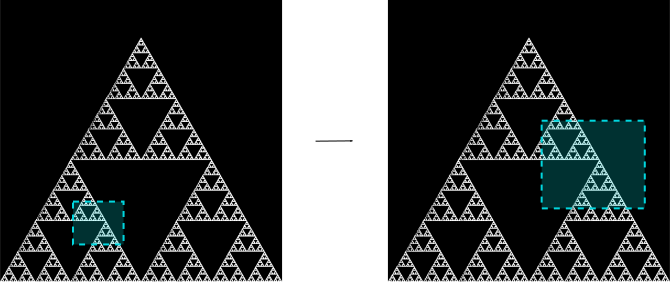
\includegraphics[width=\textwidth]{figures/sierpinsky_jump}
\caption{An example of the self-similarity jumping technique. Pictured is the Sierpi\'nsky triangle IFS (\autoref{ifs:sierpinsky}).
The viewport (pictured in cyan) on the left can be transformed to the one on the right by applying the inverse mapping $f_1^{-1}$ to it.
The resulting viewport looks the same but contains more points.}
\label{figure:sierpinsky_jump}
\end{figure}

When using a point cloud, we retain detail when zooming in up to a certain depth. In this way, a point cloud is more flexible than a 
static pixel canvas, which will already show rendering artefacts when zooming in slightly beyond its intended size.

Nonetheless, while zooming in, more and more points of the point cloud fall outside of the current camera viewport
(and thus are 'useless' for the quality of the rendered image), degrading quality beyond a certain depth more than is acceptable.

However, it follows from the self-similar nature of the IFS that we might, in certain situations,
`unnoticeably' zoom out to a shallower camera viewport of the point cloud that shows the same information of the attractor
as the original viewport, but containing more points of the point cloud.

This can be done by identifying a mapping that fully encompasses the current camera viewport, and then applying its inverse
to the viewport.
`Fully encompasses' here means that 
all corners of the unit square transformed by the inverse of the camera viewport transformation
lie inside of the unit square transformed by the mapping \footnote{A simple way to do this is to treat the unit square as a simple polygon,
and then transform all of its corner points. For the resulting two polygons, the 'even-odd rule' algorithm
\cite{haines1994point}
can be used to check whether all points of one polygon are inside the other.}.

In a similar sense, transformations \(a\) and \(b\) `overlap' if the unit square transformed by \(a\) overlaps the unit square transformed by \(b\).

See \autoref{figure:sierpinsky_jump} for an example. 

The algorithm and its inverse are specified in \autoref{algorithm:self_similarity_jump_up} and \autoref{algorithm:self_similarity_jump_down}, respectively.

\begin{algorithm}
\caption{self-similarity jump-up}
\label{algorithm:self_similarity_jump_up}
  $n$: the number of mappings the IFS consists of; \\
  $v$: the current camera's view transformation; \\
  $s$: a stack of jumps made so far; \\
  \For{$i \leftarrow [1,\ldots, n]$}{ 
    \If{isInvertible($f_i$)  and isInside($v^{-1}$, $f_i$) }{
      push($s$, $f_i$); \\
      $v = f_i^{-1} \circ v$; \\
      break; \\
    }
  }
\end{algorithm}

\begin{algorithm}
\caption{self-similarity jump-down}
\label{algorithm:self_similarity_jump_down}
  $v$: the current camera's view transformation; \\
  $s$: a stack of jumps made until now; \\
  \If{notEmpty($s$) and isOutsideUnitSquare($v^{-1}$) }{
    $f$ = pop($s$); \\
    $v = f \circ v$; \\
  }
\end{algorithm}

\subsubsection{Coloring the rendering}
\label{sec:orgf67bbda}
\label{subsection:coloring}

The simplest way of rendering an IFS attractor simply renders points that are on the attractor a different color
than the points that are not.

However, more visually pleasing methods use a \emph{color map} to e.g. indicate the density (the number of points ending up at a particular canvas location) of the attractor.
Yet more advanced methods \cite{draves2003fractal} keep track of a per-point color, based on the sequence of transformations each point has undergone.

It seems possible to combine these techinques with the `self-similarity jumping', since we keep track of which mappings we have (inversely) applied to the camera viewport:
to determine the final colors of all points that will be rendered this frame, 
all visible points' colors need to be altered by the color-mutations that each of the mappings in the stack \(s\) specified by \autoref{algorithm:self_similarity_jump_up} and \autoref{algorithm:self_similarity_jump_down} would apply.

As an example, say we are viewing the lower left leaf of a fractal fern (\autoref{ifs:barnsley_fern}) and that mapping creating the lower left leaf would make the contained points red. 
If we now `jump up' we use points from virtually the whole fern.
To make these points still look visually identical from the lower left leaf, we have to alter the points' colors so they get the same reddish hues.

\subsection{Implementation}
\label{sec:org2830548}

\begin{figure}
  \centering
  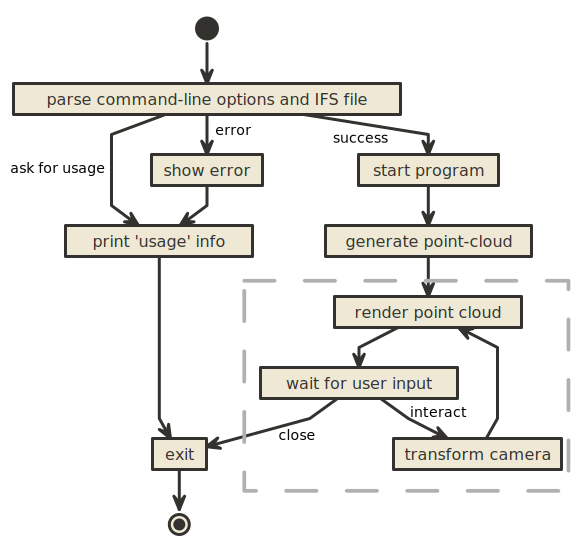
\includegraphics[width=0.5\textwidth]{figures/program_execution}
  \caption{Overview of the proof-of-concept program's execution flow. The dashed box indicates the main program loop.}
\label{figure:program_flow}
\end{figure}

The program was implemented using the general-purpose programming language Haskell, 
in combination with the GPGPU library Accelerate \cite{chakravarty2011accelerating}.
This programming stack was chosen because Accelerate 
offers a statically-typed EDSL\footnote{Embedded Domain-Specific Language.} for array-based GPGPU programming,
which is more high-level and less error-prone than writing code 
in lower-level alternatives like CUDA or OpenCL directly.\footnote{Instead of being presented with a black screen when a programming mistake is made, 
Accelerate presents errors at compile-time in many cases. Furthermore, Accelerate features a
single-threaded reference implementation that runs on the CPU that can be used to sanity-check the behaviour of code.}

The usage of Haskell as implementation language, being a pure functional language, also allowed 
the easy construction of different subcomponents making up the program,
and testing each of these independently.

A general overview of the flow of the program can be seen in \autoref{figure:program_flow}.

\subsubsection{Simplicity}
\label{sec:org69ad330}

To be able to complete the implementation within the time allotted for the thesis project,
the decision was made to keep the implementation as simple as possible.

This means that:

\begin{itemize}
\item The optimizations mentioned in \autoref{subsection:point_cloud_optimizations} were not implemented;
\item Points are rendered on screen using a simple binary mapping. (If a pixel contains one or more points, it is white; otherwise black.)
The more fancy coloring techniques outlined in \autoref{subsection:coloring} were not used.
\end{itemize}

While the program on its own might therefore not be enough to fully answer the research question,
it is able to answer the simpler question of whether the technique is at all feasible.

\subsubsection{Command-line options}
\label{sec:org41c7928}

The proof-of-concept program allows the customization of the following options

\begin{itemize}
\item `samples`: the number of points to use for the chaos game (defaults to 100,000,000)
\item `parallellism`: the number of GPU-threads to split the number of samples across (defaults to 2048)
\item `seed`: a number to seed the random number generator with. If not provided, a different arbitrary seed will be used each time.
\item `render\_width` and `render\_height` set the resolution of the program window that is displayed (defaults to \(800 \times 800\)).
\end{itemize}

\subsubsection{The `.ifs' file format}
\label{sec:org9cc2959}

The configuration language `Dhall' \cite{gonzalez2019} was used to 
easily allow a user to specify different IFSs.

The file structure allows one to indicate a list of affine transformations with associated chaos game probabilities,
as well as an initial camera view transformation.

Dhall allows the definition and re-use of variables, which can be useful
for numerical constants that are used in multiple transformations.\footnote{Unfortunately, Dhall explicitly does not allow floating-point arithmetic.
As such, one still needs to write e.g. \(1/3\) as \(0.3333333333333333\).}

An example file can be seen in \autoref{listing:barnsley_fern_ifs_file}.

The fields \(a \ldots f\) used for each of the transformations allow one to specify an affine transformation matrix of the shape

$$\begin{bmatrix} a & b & e \\ c & d & f \\ 0 & 0 & 1 \\ \end{bmatrix}.$$


\begin{lstlisting}[float, language=Haskell, frame=single, breaklines=true, basicstyle=\scriptsize\tt, captionpos=b, caption={barnsley\_fern.ifs, representing \autoref{ifs:barnsley_fern}}, label={listing:barnsley_fern_ifs_file}]
{ initialCamera =
  { a = 9.090909090909091e-2
  , b = 0.0
  , c = 0.0
  , d = -9.090909090909091e-2
  , e = 0.5
  , f = 1.0
  }
, transformations =
  [ { transformation = { a = 0.0, b = 0.0, c = 0.0, d = 0.16, e = 0.0, f = 0.0 }
    , probability = 1.0e-2
    }
  , { transformation = { a = 0.85, b = 4.0e-2, c = -4.0e-2, d = 0.85, e = 0.0, f = 1.6 }
    , probability = 0.85
    }
  , { transformation = { a = 0.2, b = -0.26, c = 0.23, d = 0.22, e = 0.0, f = 1.6 }
    , probability = 7.0e-2
    }
  , { transformation = { a = -0.15, b = 0.28, c = 0.26, d = 0.24, e = 0.0, f = 0.44 }
    , probability = 7.0e-2
    }
  ]
}

\end{lstlisting}

\subsubsection{Rendering}
\label{sec:org6f88d76}
The program computes the point cloud once, on startup, and then re-renders the image that is shown in the program window
every time the user moves the camera.

Rendering is done by iterating (in parallel) over all points in the point cloud and filling a two-dimensional histogram with the same dimensions
as the canvas with numbers. 
This histogram is then used to draw the attractor (any non-empty pixel is colored white and the rest black).

\subsubsection{Moving the camera}
\label{sec:orgb80cc47}
The camera can be moved by either zooming in or out using the scrollwheel,
or translating the camera by dragging with the mouse.

These operations alter the camera's current view transformation, 
which is stored as a transformation matrix relative to unit space.

\subsubsection{Performing 'self-similarity jumping'}
\label{sec:org087b415}

While the program is running, a user can go back to a more shallow view by pressing `+`\footnote{Strictly speaking, by pressing the `=' key; pressing SHIFT is not necessary.}, and then when inside one or multiple shallower views,
`-` can be pressed to undo the last jump.

This process was intentionally kept manual, because it allows the user to more easily compare how
the visualization looks with and without the jumping, and allows for a full exploration of the circumstances
in which a jump up is and is not actually correct (see \autoref{subsection:jumping_restrictions}).
\subsubsection{Rendering `guides'}
\label{sec:org3f4c18e}

To make it easier to see how an IFS is constructed, as well as easier for a user to orient themselves when
testing the 'self-similarity jumping', it is possible to toggle the rendering of `guides' by pressing the `g' key.
Similarly, the rendering of points can be toggled by pressing the `p' key (allowing one to see the guides more clearly, when desired).

These 'guides' are the unit square, after undergoing a sequence of zero, one, two etc. mappings of the IFS.
Different colors are used for guides at different sequence-depths.

\begin{figure}
     \centering
     \begin{subfigure}[b]{0.3\textwidth}
         \centering
         
\includegraphics[width=\textwidth]{figures/barnsley_points}
         \caption{only points}
         \label{figure:barnsley_points}
     \end{subfigure}
     \hfill
     \begin{subfigure}[b]{0.3\textwidth}
         \centering
         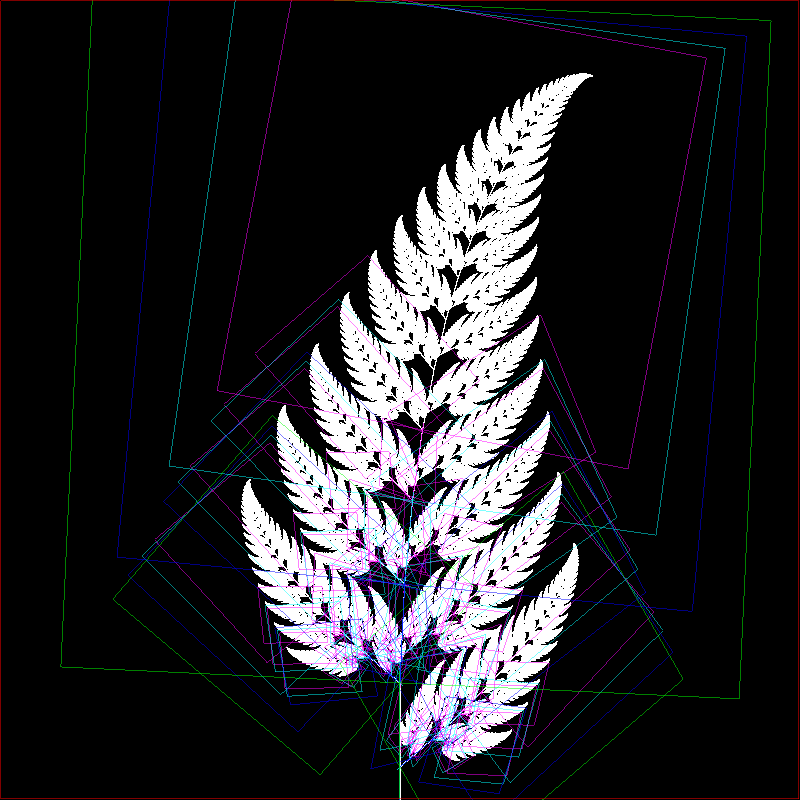
\includegraphics[width=\textwidth]{figures/barnsley_guides_and_points}
         \caption{guides and points}
         \label{figure:barnsley_guides_and_points}
     \end{subfigure}
     \hfill
     \begin{subfigure}[b]{0.3\textwidth}
         \centering
         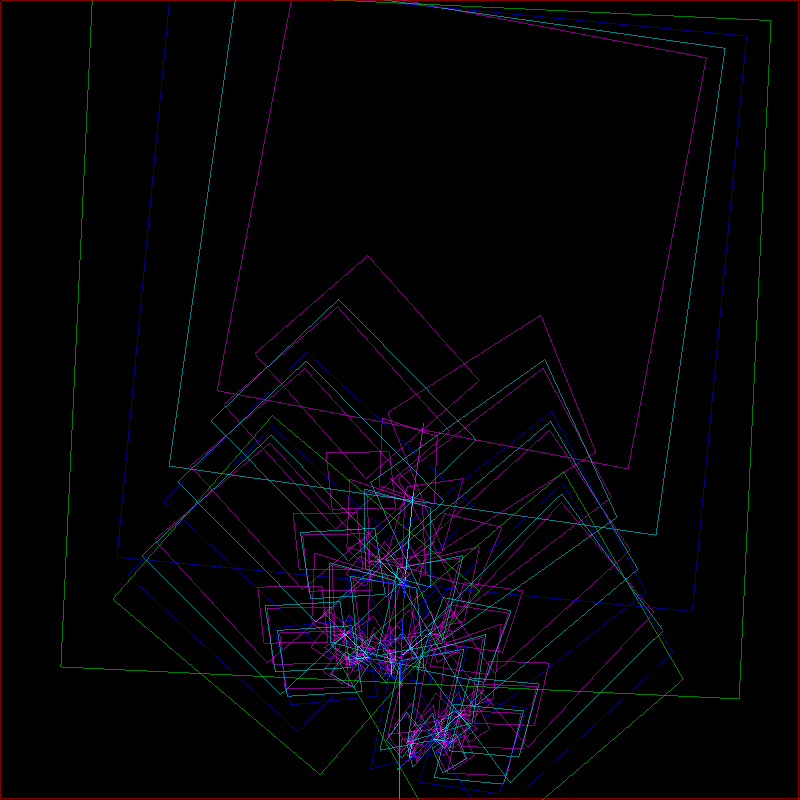
\includegraphics[width=\textwidth]{figures/barnsley_guides}
         \caption{only guides}
         \label{figure:barnsley_guides}
     \end{subfigure}
        \caption{The Barnsley Fern (\autoref{ifs:barnsley_fern}) rendered by the program in different ways.}
        \label{figure:barnsley_guides_vs_points}
\end{figure}

\section{Findings}
\label{sec:org398ff7e}
\label{section:findings}

\subsection{Restrictions on `self-similarity jumping'}
\label{sec:org65f2efd}
\label{subsection:jumping_restrictions}

From experimentation with the program it turns out that there are two common situations
in which the technique outlined in \autoref{subsection:self_similarity} cannot be used.

\begin{enumerate}
\item Borders between transformations
\label{sec:org8cd0fea}

It is rather common to zoom in on the borders between two regions of points, where each region contains points that have had a different transformation applied to them as most recent one. 
This is often where interesting visual details of the IFS might appear.

However, \autoref{algorithm:self_similarity_jump_up} is not able to handle these `borders' between transformation regions,
as the camera `overlaps multiple mapping regions' (using the definition of subsection:self\textsubscript{similarity}),
it is contained in neither and therefore the algorithm cannot fine a self-similarity to jump up to even if there is one.

An example can be seen in figure \autoref{figure:sierpinsky_transformation_borders}.

\begin{figure}
\centering
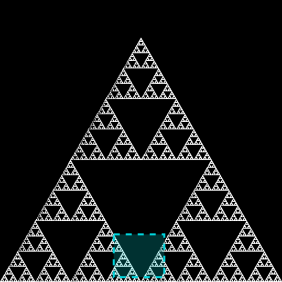
\includegraphics[width=0.3\textwidth]{figures/sierpinsky_transformation_borders}
\caption{In this example the camera viewport (indicated in cyan) overlaps (as defined in \autoref{subsection:self_similarity}) both $f_1$ and $f_2$ of \autoref{ifs:sierpinsky} partially. This case is not handled by \autoref{algorithm:self_similarity_jump_up}. }
\label{figure:sierpinsky_transformation_borders}
\end{figure}

\item Overlapping subtransformations
\label{sec:org46123c8}

\begin{figure}
     \centering
     \begin{subfigure}[b]{\textwidth}
         \centering
         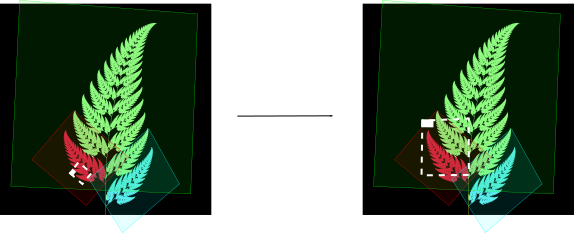
\includegraphics[width=0.6\textwidth]{figures/barnsley_colored_jump1}
         \caption{Since the camera viewport only contains points of $f_2$, the jump up is proper.}
         \label{figure:barnsley_jump_a}
     \end{subfigure}
     \hfill
     \begin{subfigure}[b]{\textwidth}
         \centering
         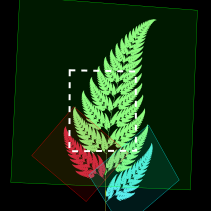
\includegraphics[width=0.6\textwidth]{figures/barnsley_colored_jump2}
         \caption{Since the camera viewport contains both points of $f_2$ and $f_3$, the jump is incorrect. 
Note that the leaf in the lower left is missing after the jump.}
         \label{figure:barnsley_jump_b}
     \end{subfigure}
        \caption{Problems when jumping up on \autoref{ifs:barnsley_fern}. 
The mappings $f_1$, $f_2$ and $f_3$ refer to the mappings of \autoref{ifs:barnsley_fern}. 
The top row of a) and b) is `world space' with the camera viewport indicated as white dashed polygon. 
The bottom rows show the camera viewport.
Points are colored based on their latest mapping. }
        \label{figure:barnsley_jump}
\end{figure}

A more shallow view of the attractor only actually is self-similar to the current view when
there are no points transformed by another mapping that end up in the current view.

\todo[inline]{Better explain paragraph above}

When there are points from another mapping in the current view, 
going to a more shallow view will make points disappear from the perspective of the user.
In practice, this means that for many IFSs there are large regions in which the technique cannot be used.

Simple IFSs like the Sierpińsky Triangle (\autoref{ifs:sierpinsky}) in which transformations
do not overlap\footnote{As defined in \autoref{subsection:self_similarity}.}, do not exhibit this problem. 
Slightly more complex IFSs like the Dragon Curve (\autoref{ifs:dragon_curve}) or the Barnsley Fern (\autoref{ifs:barnsley_fern}) however do.

See \autoref{figure:barnsley_jump} for an example 
and \autoref{figure:dragon_curve_overlaps} for a graphical explanation of what regions overlap.


This case is annoyingly common and there is no clear solution to alleviate this restriction.
Furthermore, it is not simple to check whether we are currently in a region that exhibits the problem,
as this would require evaluating the IFS itself.

It is possible to take a rough `upper bound' estimate of the disallowed regions by keeping track, 
per mapping \(f_i\), what region would be covered by 
taking the union of transforming the unit square by all \$k\$-long sequences of mappings that start with \(f_i\).
This estimate increases in precision as \(k\) grows.

where the unit square would end up after a few transformation steps with this mapping as last (i.e. most significant) one.


\begin{figure}
     \centering
     \begin{subfigure}[b]{0.4\textwidth}
         \centering
         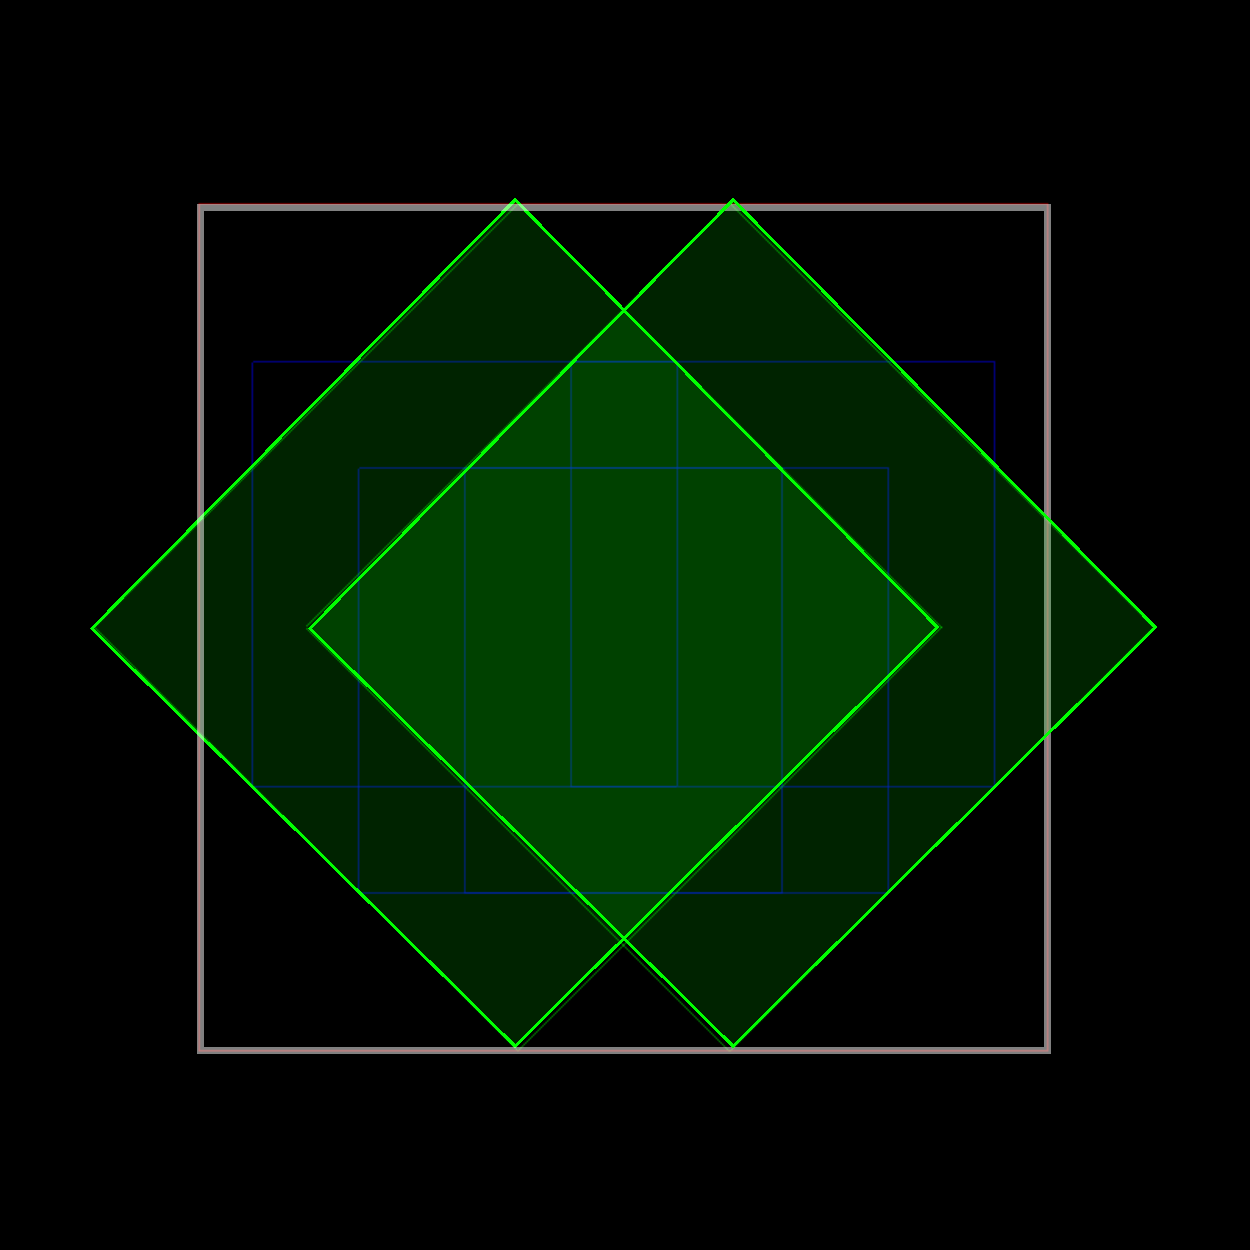
\includegraphics[width=\textwidth]{figures/dragon_curve_a}
         \caption{The unit square (indicated in white) transformed by $f_1$ and $f_2$ (indicated in green)}
         \label{figure:dragon_curve_a}
     \end{subfigure}
     \hfill
     \begin{subfigure}[b]{0.4\textwidth}
         \centering
         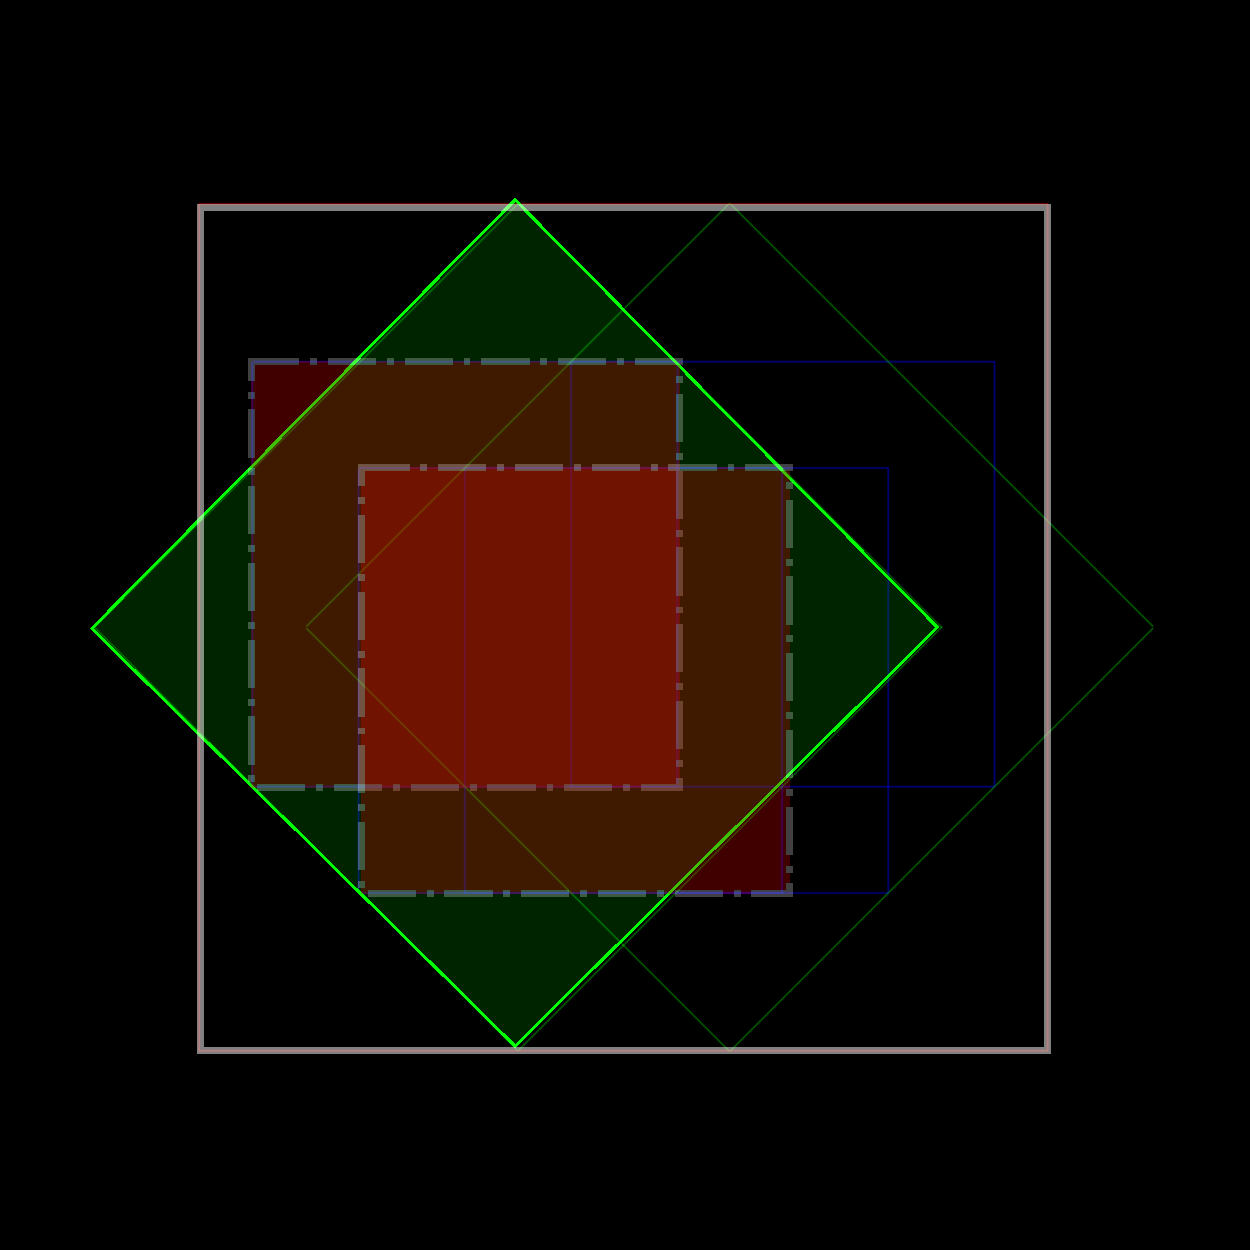
\includegraphics[width=\textwidth]{figures/dragon_curve_b}
         \caption{Subtransformations of $f_1$: $f_1 \circ f_1$ and $f_1 \circ f_2$ (indicated in shades of red)}
         \label{figure:dragon_curve_b}
     \end{subfigure}
     \hfill
     \begin{subfigure}[b]{0.4\textwidth}
         \centering
         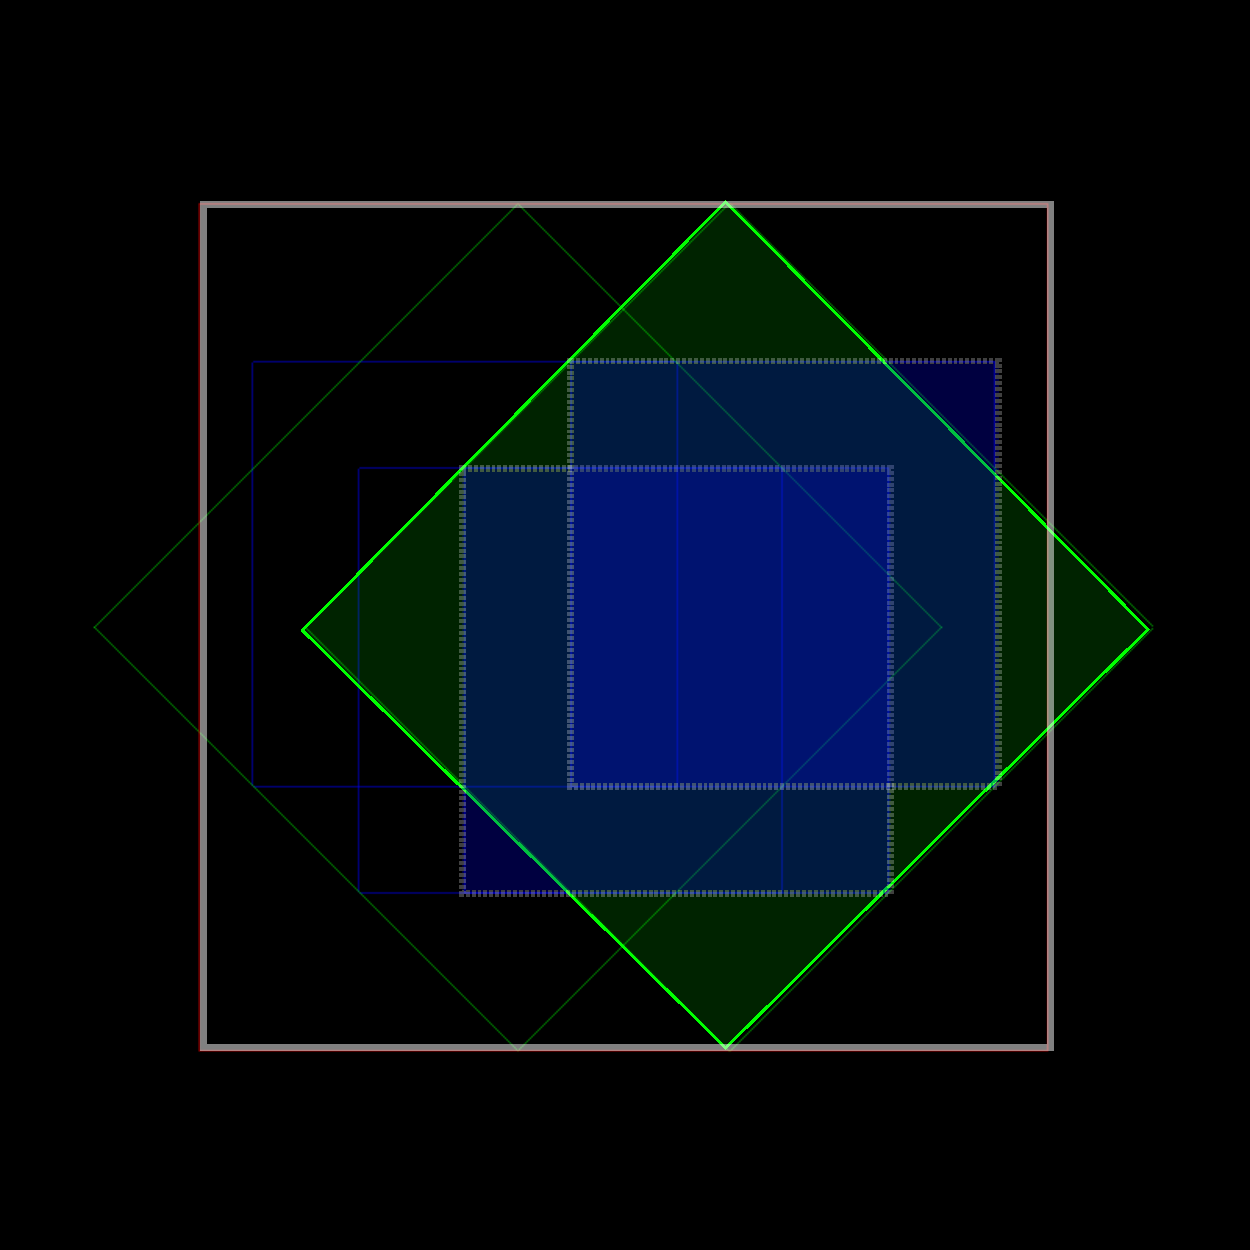
\includegraphics[width=\textwidth]{figures/dragon_curve_c}
         \caption{Subtransformations of $f_2$: $f_2 \circ f_1$ and $f_2 \circ f_2$. (indicated in shades of blue)}
         \label{figure:dragon_curve_c}
     \end{subfigure}
     \hfill
     \begin{subfigure}[b]{0.4\textwidth}
         \centering
         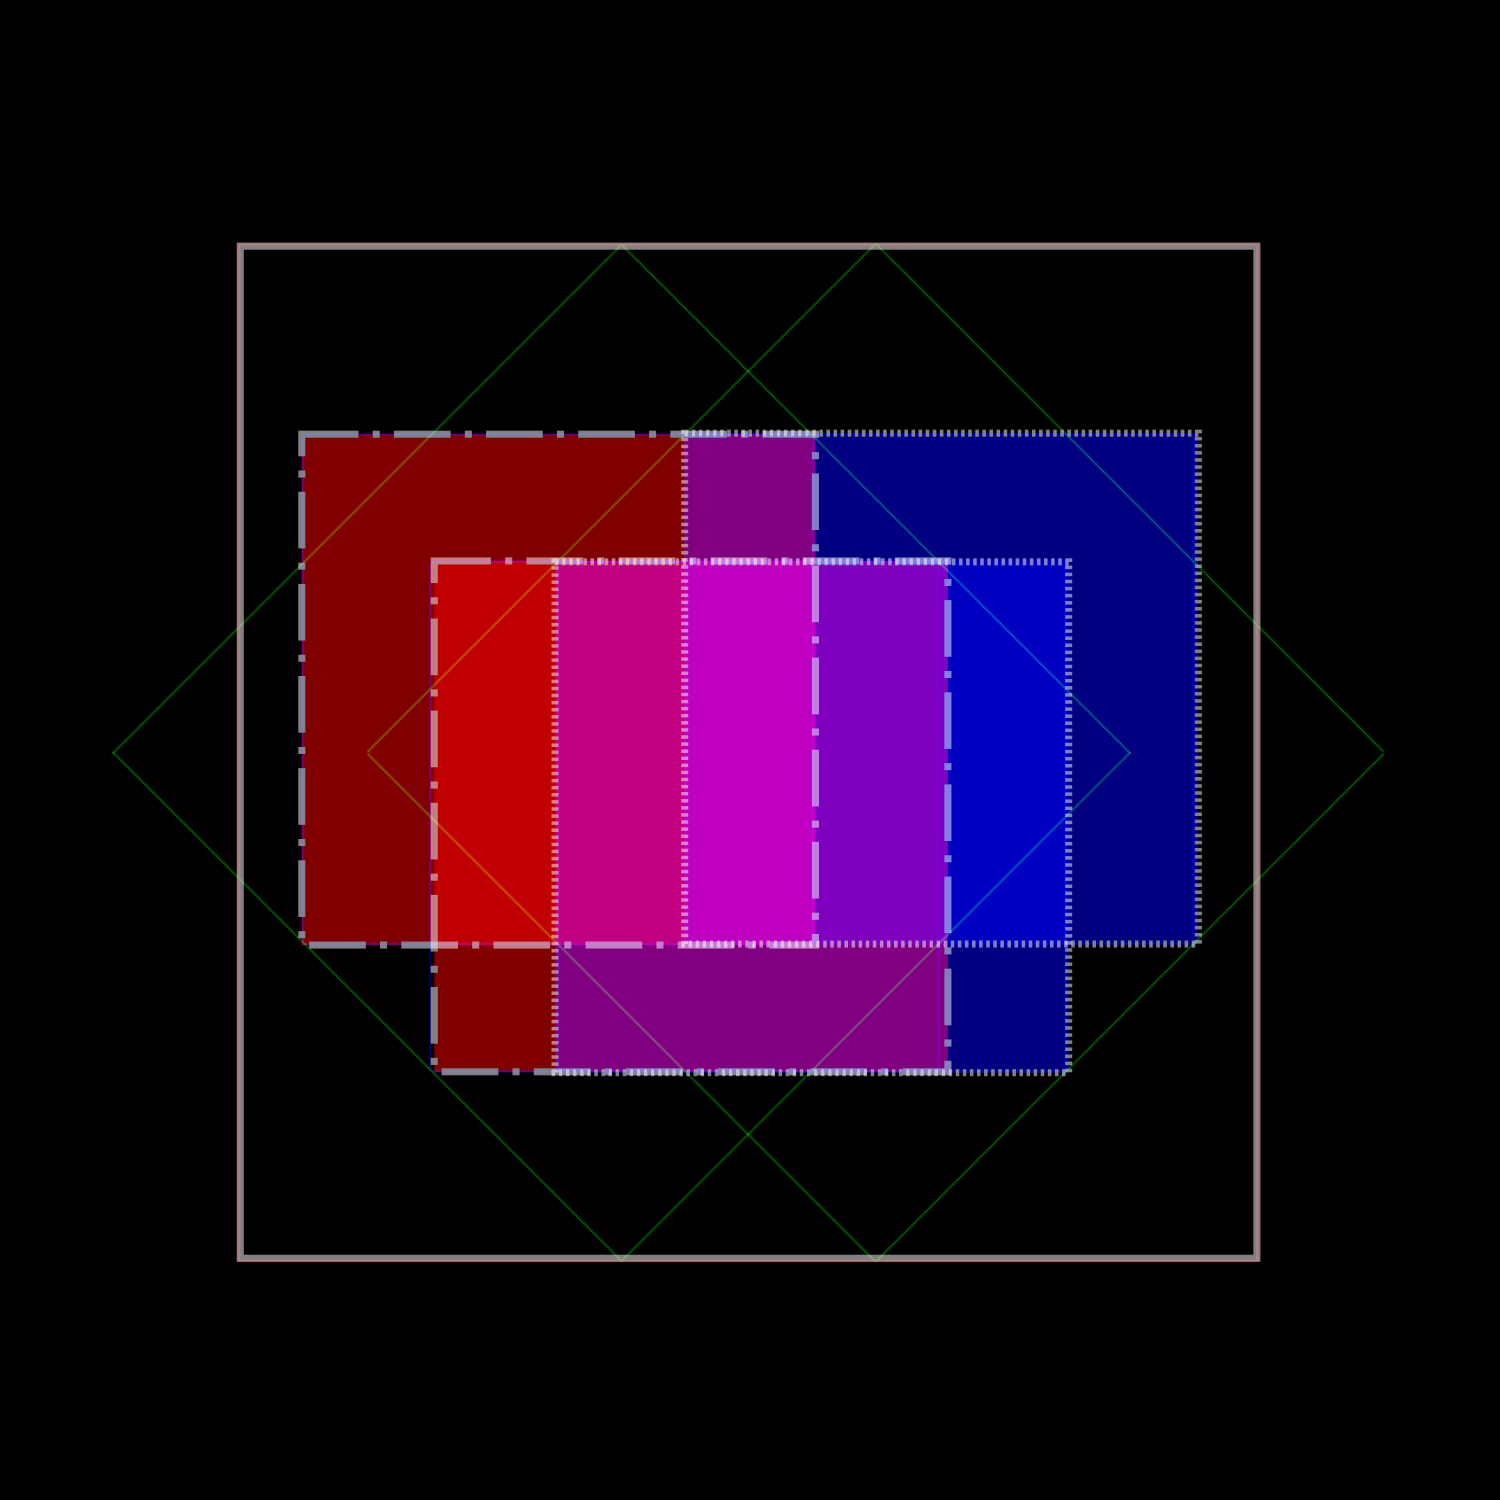
\includegraphics[width=\textwidth]{figures/dragon_curve_d}
         \caption{The region in which (b) and (c) overlap, indicated in shades of magenta)}
         \label{figure:dragon_curve_d}
     \end{subfigure}
        \caption{Showing the first couple of iterations of rendering the attractor of the dragon curve IFS $D$ (\autoref{ifs:dragon_curve}), and the regions in which (sequences of) transformations overlap (As defined in \autoref{subsection:self_similarity}).}
        \label{figure:dragon_curve_overlaps}
\end{figure}

\todo[inline]{Increase whitespace between subfigures}
\end{enumerate}

\subsection{Memory Usage}
\label{sec:org6a4f19c}

Point clouds take up a lot of memory on the GPU. To render a fractal at reasonable detail, depending on the particular IFS,
hundreds of millions if not billions of points are necessary.

A reasonable way to store a point cloud is by using 32 bits for each of the two coordinates of a point. 
This means that one point takes up exactly one machine word of a 64-bit computer system.
Stored this way, a point cloud of 100,000,000 points requires 0.596 GiB of GPU memory,
and 1,000,000,000 points requires 5.96 GiB.
For current generation GPUs\footnote{At the time of writing, high-end consumer GPUs contain somewhere between 2 and 24 GiB of available memory \cite{ign2020topgpus}.}, this often is more memory than available.

\todo[inline]{Elaborate claim. `The latter only'? (see feedback)}

\section{Conclusion}
\label{sec:orga792377}
\label{section:conclusion}

A program was implemented which has shown that there is \emph{some} merit to rendering an IFS's attractor using a point cloud as re-usable intermediate structure.
However, the self-similarity detection method that was proposed turns out to be unusable in common cases.

Therefore, the proposed technique can be considered of limited practicality, 
at least until a more sophisticated self-similarity detection method is found.

\section{Future Work}
\label{sec:org6a08dfe}
\label{section:further_work}

It is our hope that a more sophisticated way of detecting self-similarity might be found,
which would make `self-similarity jumping' more practical.

Besides this, while we have shown in a proof-of-concept program that it is possible to render an IFS using a point cloud,
there are many optimizations that could be made to make the program run faster (potentially even in real-time),
most notably the rendering optimizations listed in \autoref{subsection:point_cloud_optimizations}.

Another venue that could be explored is the rendering of an IFS's attractor at multiple `levels of detail':
It might be possible to create more detailed local versions of the point cloud (based on the points of the less detailed point cloud) when the user
zooms in on a particular region, on demand.

Finally it is worth noting that \cite{lawlor2012gpu} already presents an efficient way to render 
a large set of IFSs using a very different approach (c.f. \autoref{subsection:deterministic_gpu}), 
which might be worthwhile to be explored further.

\pagebreak
\printbibliography
\clearpage

\appendix

\section{Iterated Function Systems used}
\label{sec:org7ad83de}

This appendix lists the mapping functions of the IFSs that were used throughout this thesis.
The \(p\)-values next to each of the mappings references the probability that this mapping ought to be chosen,
if a chaos game-based rendering method is used (c.f. \autoref{subsection:chaos_game}).


\begin{ifs}
\centering
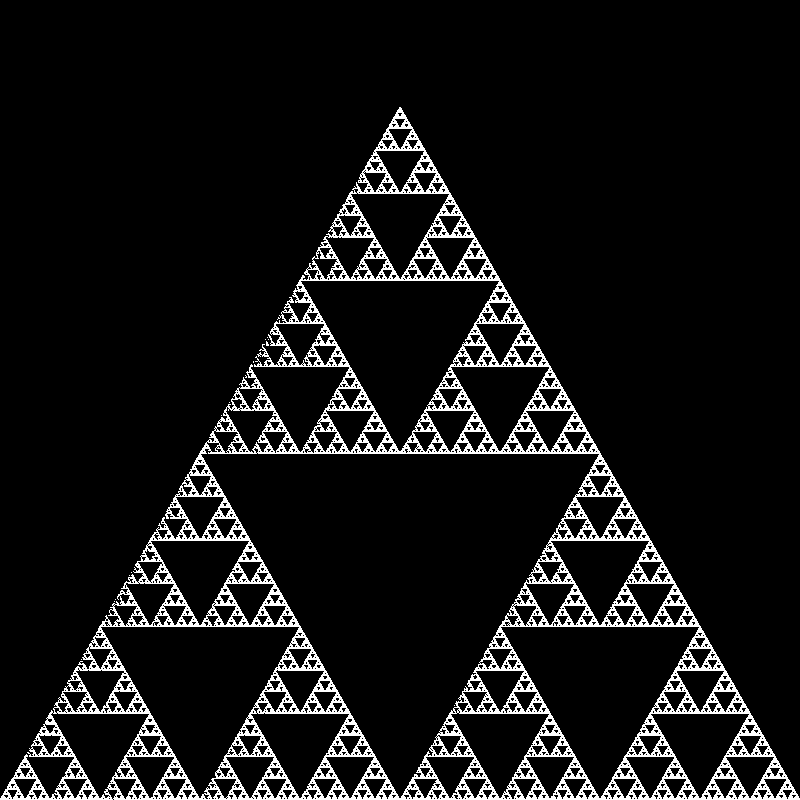
\includegraphics[width=0.2\textwidth]{figures/sierpinsky}
$$ 
\begin{aligned}
f_1(x, y) &= \begin{bmatrix} \frac{1}{2} & 0 \\ 0 & \frac{1}{2} \end{bmatrix} & \begin{bmatrix} x \\ y \end{bmatrix} & , &p_1 = \frac{1}{3} \\
f_2(x, y) &= \begin{bmatrix} \frac{1}{2} & 0 \\ 0 & \frac{1}{2} \end{bmatrix} & \begin{bmatrix} x \\ y \end{bmatrix} &+ \begin{bmatrix} \frac{1}{2} \\ 0 \end{bmatrix} , &p_2 = \frac{1}{3} \\
f_3(x, y) &= \begin{bmatrix} \frac{1}{2} & 0 \\ 0 & \frac{1}{2} \end{bmatrix} & \begin{bmatrix} x \\ y \end{bmatrix} &+ \begin{bmatrix} \frac{1}{4} \\ \frac{\sqrt{3}}{4} \end{bmatrix} , &p_3 = \frac{1}{3} \\
\end{aligned}
$$

\caption{the Sierpi\'nsky triangle}
\label{ifs:sierpinsky}
\end{ifs}

\begin{ifs}
\centering
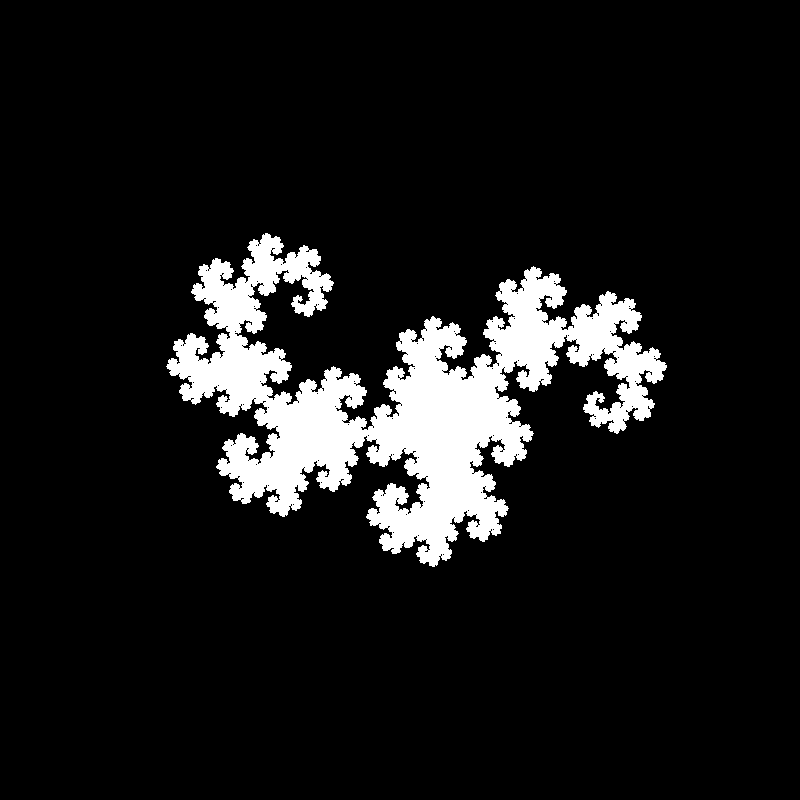
\includegraphics[width=0.2\textwidth]{figures/dragon_curve}
$$ 
\begin{aligned}
f_1(x,y) &= \frac{1}{\sqrt{2}}\begin{bmatrix} \cos 45^\circ & -\sin 45^\circ \\ \sin 45^\circ & \cos 45^\circ \end{bmatrix} & \begin{bmatrix} x \\ y \end{bmatrix} & , &p_1 = \frac{1}{2} \\
f_2(x,y) &= \frac{1}{\sqrt{2}}\begin{bmatrix} \cos 135^\circ & -\sin 135^\circ \\ \sin 135^\circ & \cos 135^\circ \end{bmatrix} & \begin{bmatrix} x \\ y \end{bmatrix} &+ \begin{bmatrix} 1 \\ 0 \end{bmatrix} , &p_2 = \frac{1}{2} \\
\end{aligned}
$$

\caption{the Heighway Dragon Curve}
\label{ifs:dragon_curve}
\end{ifs}

\begin{ifs}
\centering

\includegraphics[width=0.2\textwidth]{figures/barnsley_100000000}
$$ 
\begin{aligned}
f_1(x,y) &= \begin{bmatrix} \ 0.00 & \ 0.00 \ \\ 0.00 & \ 0.16 \end{bmatrix}  & \begin{bmatrix} \ x \\ y \end{bmatrix} & , &p_1 = 0.01 \\
f_2(x,y) &= \begin{bmatrix} \ 0.85 & \ 0.04 \ \\ -0.04 & \ 0.85 \end{bmatrix} & \begin{bmatrix} \ x \\ y \end{bmatrix} &+ \begin{bmatrix} \ 0.00 \\ 1.60 \end{bmatrix} , &p_2 = 0.85 \\
f_3(x,y) &= \begin{bmatrix} \ 0.20 & \ -0.26 \ \\ 0.23 & \ 0.22 \end{bmatrix} & \begin{bmatrix} \ x \\ y \end{bmatrix} &+ \begin{bmatrix} \ 0.00 \\ 1.60 \end{bmatrix} , &p_3 = 0.07 \\
f_4(x,y) &= \begin{bmatrix} \ -0.15 & \ 0.28 \ \\ 0.26 & \ 0.24 \end{bmatrix} & \begin{bmatrix} \ x \\ y \end{bmatrix} &+ \begin{bmatrix} \ 0.00 \\ 0.44 \end{bmatrix} , &p_4 = 0.07 \\
v(x, y) &= \begin{bmatrix} 0.09 & \ 0.00 \\ 0.00 & \ -0.09 \end{bmatrix} & \begin{bmatrix} \ x \\ y \end{bmatrix} &+ \begin{bmatrix} \ 0.50 \\ 1.00 \end{bmatrix} \\
\end{aligned}
$$
\caption{the Barnsley Fern}
\label{ifs:barnsley_fern}
\end{ifs}
\end{document}